\documentclass[tikz,border=4pt]{standalone}
\usepackage[T1]{fontenc}
\usepackage{lmodern}
\usetikzlibrary{arrows.meta,calc,positioning}
\ifdefined\darkmode
  \definecolor{paper}{HTML}{17191B}\definecolor{ink}{HTML}{D7D7D3}
  \definecolor{muted}{HTML}{969A9C}\definecolor{accent}{HTML}{7F9EAE}
  \definecolor{solar}{HTML}{C4A56C}\definecolor{line}{HTML}{3B4043}
  \definecolor{panel}{HTML}{202326}
\else
  \definecolor{paper}{HTML}{F5F5F2}\definecolor{ink}{HTML}{202326}
  \definecolor{muted}{HTML}{666B70}\definecolor{accent}{HTML}{315F78}
  \definecolor{solar}{HTML}{8A6428}\definecolor{line}{HTML}{CFD2D2}
  \definecolor{panel}{HTML}{ECEEEC}
\fi
\begin{document}\sffamily
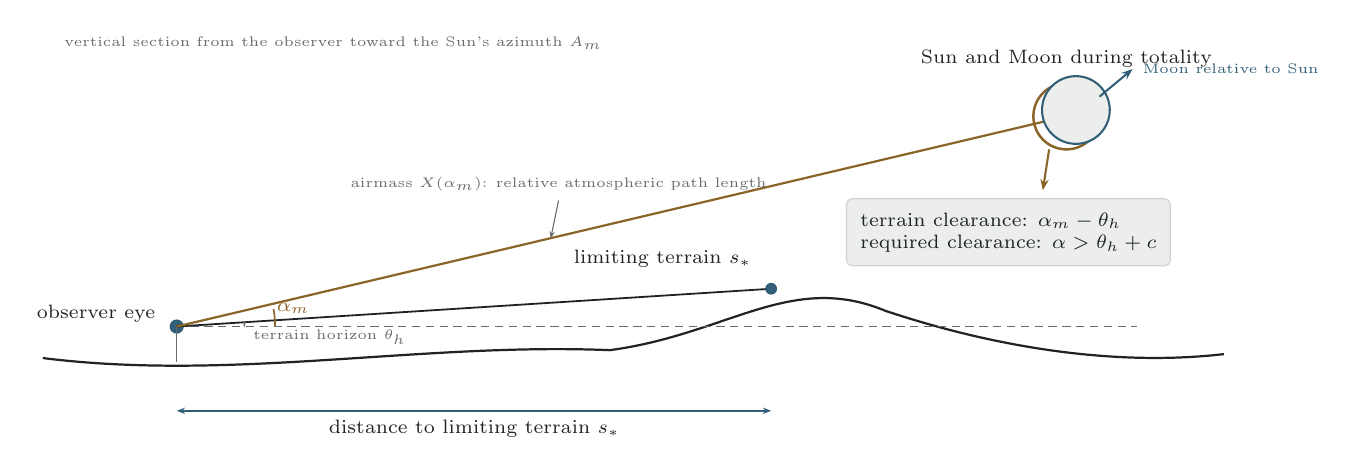
\begin{tikzpicture}[x=1cm,y=1cm,
  label/.style={text=ink,font=\scriptsize},
  note/.style={text=muted,font=\tiny,align=center},
  ray/.style={draw=solar,line width=.8pt},
  moonvector/.style={draw=accent,line width=.75pt,-{Stealth[length=4pt]}},
  solarvector/.style={draw=solar,line width=.75pt,-{Stealth[length=4pt]}},
  dim/.style={draw=accent,line width=.55pt,{Stealth[length=3pt]}-{Stealth[length=3pt]}}
]
\node[note,anchor=west] at (.15,5.15)
  {vertical section from the observer toward the Sun's azimuth $A_m$};
\draw[ink,line width=.8pt]
  (0,1.15) .. controls (2.4,.85) and (4.8,1.35) .. (7.2,1.25)
  .. controls (8.7,1.45) and (9.5,2.25) .. (10.7,1.75)
  .. controls (12.2,1.25) and (13.7,1.05) .. (15,1.2);
\coordinate (eye) at (1.7,1.55);
\coordinate (ridge) at (9.25,2.03);
\coordinate (sun) at (13.0,4.22);
\fill[accent] (eye) circle (.09);
\draw[muted,line width=.55pt] (1.7,1.1)--(eye);
\node[label,anchor=east] at (1.55,1.72) {observer eye};
\draw[muted,densely dashed,line width=.45pt] (eye)--++(12.2,0);
\draw[ink,line width=.65pt] (eye)--(ridge);
\draw[ray] (eye)--(sun);
\fill[accent] (ridge) circle (.075);
\node[label,anchor=south east] at (9.12,2.18) {limiting terrain $s_*$};
\draw[solar,line width=.9pt] (sun) circle (.42);
\fill[panel,draw=accent,line width=.75pt] ($(sun)+(.12,.08)$) circle (.43);
\node[label,anchor=south] at (13.0,4.72) {Sun and Moon during totality};
\draw[moonvector] ($(sun)+(.42,.25)$)--++(.42,.35)
  node[text=accent,font=\tiny,anchor=west] {Moon relative to Sun};
\draw[solarvector] ($(sun)+(-.22,-.42)$)--++(-.08,-.52)
  node[text=solar,font=\tiny,anchor=north] {Sun descends};
\node[note,anchor=south] (airmass) at (6.55,3.15)
  {airmass $X(\alpha_m)$: relative atmospheric path length};
\draw[muted,line width=.4pt,-{Stealth[length=2.5pt]}]
  (airmass.south)--(6.45,2.67);
\draw[solar,line width=.6pt] ($(eye)+(1.25,0)$) arc (0:10.3:1.25);
\node[text=solar,font=\scriptsize] at (3.18,1.78) {$\alpha_m$};
\draw[muted,line width=.6pt] ($(eye)+(.86,0)$) arc (0:3.7:.86);
\node[note,anchor=west] at (2.55,1.42) {terrain horizon $\theta_h$};
\draw[dim] (1.7,.48)--(9.25,.48);
\node[label] at (5.48,.25) {distance to limiting terrain $s_*$};
\node[draw=line,fill=panel,rounded corners=2pt,text=ink,font=\scriptsize,
  align=left,anchor=north west,inner sep=5pt] at (10.2,3.18)
  {terrain clearance: $\alpha_m-\theta_h$\\
   required clearance: $\alpha>\theta_h+c$};
\end{tikzpicture}
\end{document}
